\chapter*{Lab 6 - Shaders}

\section{Wave Motion}
Per questa applicazione era richiesto di implementare tre punti:
\begin{itemize}
  \item usando il tempo e data l'ampiezza e la frequenza, si richiedeva di applicare una perturbazione su asse y ad ogni vertice dell'oggetto utilizzando una certa formula
  \item al click sinistro, modificare l'ampiezza
  \item al click destro modificare la frequenza
\end{itemize}
Il primo punto è stato applicato nel file \texttt{v.glsl} poiché si tratta di un modifica a livello di vertice. Si è semplicemente applicata la formula al vertice utilizzando \texttt{gl\_Vertex} per ottenere la posizione del vertice e \texttt{gl\_Position} per fornirgli la nuova generata dalla formula.

Le modifiche successive riguardano il file \texttt{wave.c}. Attraverso \texttt{glGetUniformLocation}, nella \texttt{init} si ottengono i valori di ampiezza, frequenza e tempo. Mentre nella \texttt{keyboard}, attraverso la \texttt{glUniform1f} si fornisce al vertice un nuovo valore di frequenza o di ampiezza a seconda del click dell'utente. Il valore randomico viene ottenuto grazie alla selezione casuale di un indice del vettore \texttt{values} che contiene i valori forniti dal testo.\\
Di seguito, il risultato:
 \begin{figure}[htb]
    \centering
    %\vspace{-0.7cm}
    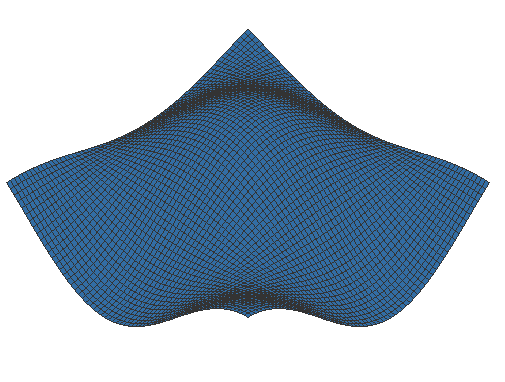
\includegraphics[width=0.7\textwidth]{wave}
    \caption{\label{fig:wave}}
    %\vspace{-0.3cm}
\end{figure}
 
\section{Particle System}
L'applicazione del sistema particellare richiedeva di:
\begin{itemize}
  \item modificare dimensione delle particella a seconda dell'altezza
  \item muovere le particelle anche nella direzione dell'asse z.
\end{itemize}

\begin{wrapfigure}{l}{0.4\textwidth} %this figure will be at the right
    \centering
    %\vspace{-1.3cm}
    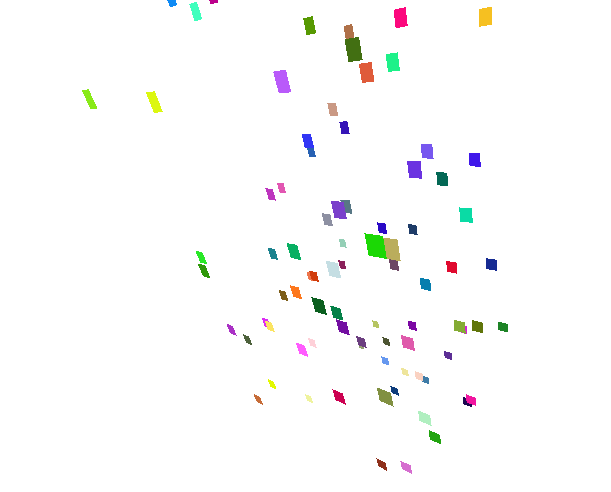
\includegraphics[height=5.5cm]{particle}
    \caption{\label{fig:particle}}
    %\vspace{-1.3cm}
\end{wrapfigure}

Il primo punto è stato implementato modificando la \texttt{gl\_PointSize} a livello di vertex. Per farlo è necessario abilitare \texttt{GL\-\_POINT\-\_SPRITE} e \texttt{GL\-\_VERTEX\-\_PROGRAM\-\_POINT\-\_SIZE} e assegnarli un valore composto dal contributo della posizione del vertice negli assi \texttt{y} e \texttt{z}.\\

Il secondo punto invece richiedeva l'elaborazione dell'attributo \texttt{vzParam} e di gestire la condivisione di esso con tutti i vertex.  È stato quindi gestito attraverso le funzioni \texttt{glGetAttribLocation} nella \texttt{init} per ottenere la possibilità di modificarlo e \texttt{glVertexAttrib1f} nella \texttt{draw} per poterlo modificare effettivamente con la velocità del vettore \texttt{velocity}.


\section{Phong Lighting}
L'obiettivo della terza applicazione è quello di creare un terzo shader che utilizzi il vero raggio riflesso e non l'Half-Way. A livello di vertex si è quindi ricavato il raggio riflesso R attraverso la funzione \texttt{reflect} tra L e N. A livello di fragment si sostituisce Half con il vettore Ray appositamente creato (fornendogli anche un fattore di shininess diverso per marcare le differenze tra i due modelli). \\
Per quanto riguarda il secondo punto, che richiedeva di rappresentare i tre diversi modelli in un'unica scena, è stata modificata la \texttt{draw} in modo da disegnare tre teapot identiche, ma con l'abilitazione di uno dei 3 diversi shader per ogni teapot. È stata inoltre allargata la finestra ed eliminata la gestione della tastiera poiché non serve più cambiare tipo di shader alla pressione dei tasti 1,2,3 in quanto i modelli sono tutti disegnati contemporaneamente.
Un esempio del risultato:
 \begin{figure}[htb]
    \centering
    %\vspace{-0.7cm}
    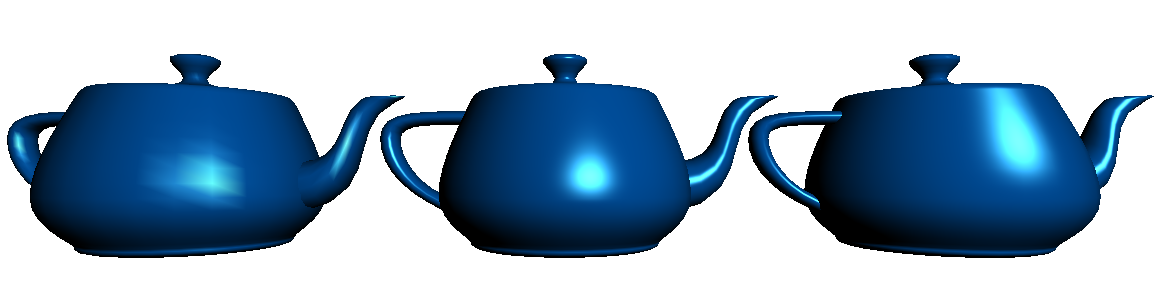
\includegraphics[width=\textwidth]{phong}
    \caption{\label{fig:phong}}
    %\vspace{-0.3cm}
\end{figure}

\section{Toon Shading}
La quarta applicazione richiedeva di disegnare un'outline sulla teapot in stile cartone animato.\\

\begin{wrapfigure}{r}{0.3\textwidth} %this figure will be at the right
    \centering
    \vspace{-0.5cm}
    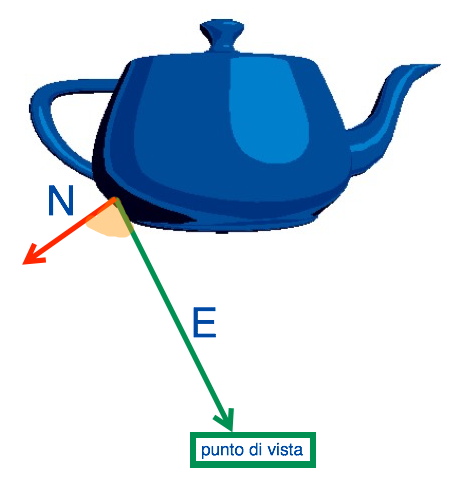
\includegraphics[height=4cm]{angle}
    \caption{\label{fig:angle}}
    \vspace{-0.3cm}
\end{wrapfigure}
L'idea di base è quella di cambiare colore ai vertici la cui normale forma un angolo maggiore di un certo angolo con il vettore che congiunge vertice e punto di vista. Quindi occorre ottenere per ogni vertex, il vettore E che va dal punto di vista al vertex stesso e ottenere l'angolo utilizzando l'arcocoseno del prodotto scalare tra questi due vettori normalizzati.
Il vettore E viene ottenuto a livello di vertex, mentre a livello di fragment si calcola l'angolo e si applica il colore se quest'ultimo supera un certo angolo, ad esempio 74\degree. La funzione \texttt{acos} prende in ingresso un valore compreso tra 0 e $\pi$, quindi per rappresentare i 74 gradi è necessario passargli $3.14/10*4.1$ ovvero $180/10*4.1=73.8$.\\

Due esempi del risultato:
\begin{figure}[hbt]
    \centering
    \vspace{-0.5cm}
    \subfloat[74\degree, rosso]{{
\includegraphics[height=3cm]{toon1} }}%
    \subfloat[80\degree, nero con altre modifiche colore]{{
\includegraphics[height=3cm]{toon2} }}%
	\vspace{-0.5cm}
\end{figure}

\section{Morphing}
In questa applicazione era richiesto di applicare il colore al triangolo e variare il colore in funzione del tempo. In alternativa era possibile modificare la forma da triangolo a quadrato. Sono state implementate entrambe le interpolazioni tra colore e forme. A livello di vertex, è stato aggiunto il vettore dei colori che deve assumere il quadrato ed è stata modificata la modalità con cui viene fornito il colore al vertice: analogamente ai vertici, si è utilizzata la funzione \texttt{mix} tra il colore corrente e il colore finale a seconda del tempo.
Nel sorgente C, è stata modificata la funzione \texttt{draw} in modo che disegnasse quadrati (\texttt{GL\_QUAD}) e all'interno, per ogni vertice del quadrato:
\begin{itemize}
  \item si fornisce il colore del vertice
  \item si fornisce al vertex, la posizione finale e il colore finale
  \item si disegna il vertice iniziale
\end{itemize}

La figura iniziale viene rappresentata come triangolo, ma in realtà un quadrato con due vertici coincidenti. Attraverso l'interpolazione, i due vertici divergono e vanno a posizionarsi in modo da formare il quadrato finale.\\
\newpage
Il risultato finale:
\begin{figure}[hbt]
    \centering
    \vspace{-0.5cm}
    \subfloat[Triangolo iniziale]{{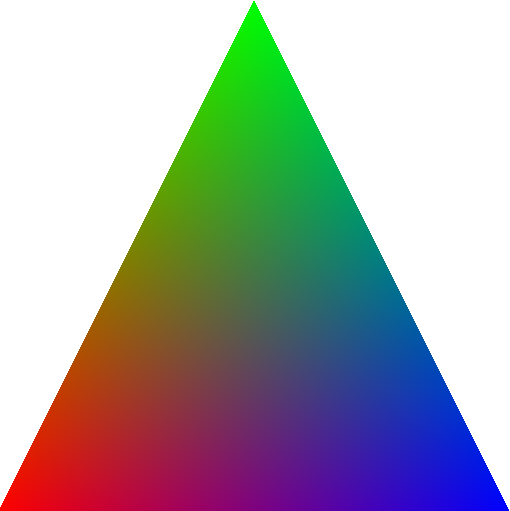
\includegraphics[height=4cm]{morph1.png} }}%
    \subfloat[Durante l'interpolazione]{{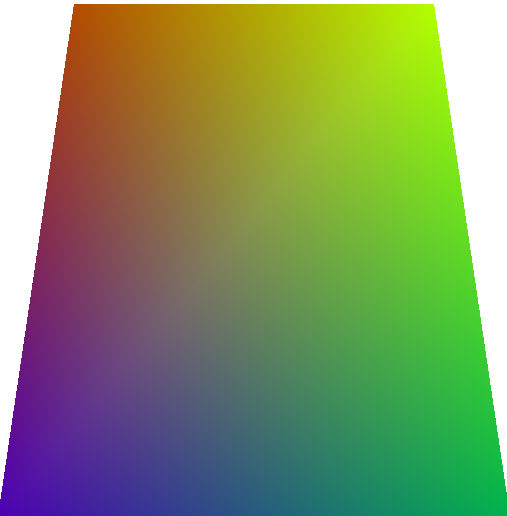
\includegraphics[height=4cm]{morph2.png} }}%
    \subfloat[Quadrato finale]{{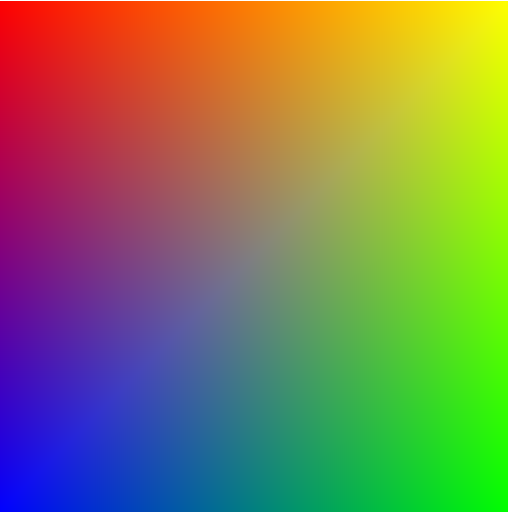
\includegraphics[height=4cm]{morph3.png} }}%
\end{figure}


\section{Bump Mapping}
\begin{wrapfigure}{r}{0.4\textwidth} %this figure will be at the right
    \centering
    \vspace{-1.5cm}
    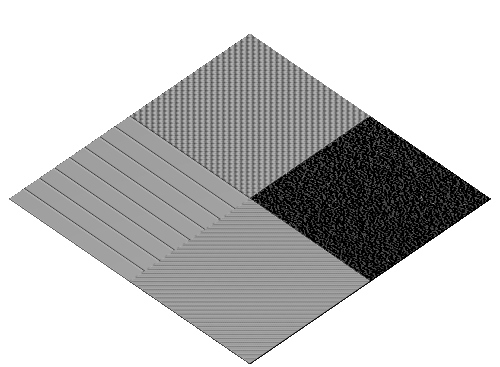
\includegraphics[height=5.5cm]{bump}
    \caption{\label{fig:bump}}
    \vspace{-2cm}
\end{wrapfigure}
L'obiettivo di questa applicazione era modificare l'input data per ottenere un effetto particolare di bump mapping sulla superficie. È stato quindi diviso il quadrato in quattro parti, ognuna con un particolare valore randomizzato o ottenuto tramite seni, coseni o modulo. Il risultato è il seguente:


\vspace{3cm}
\section{Cube environment mapping}
Nell'ultimo esercizio era richiesto di sostituire i colori del cubo con immagini ed applicare l'environment cube mapping.
Sono state scelte sei immagini dell'esercitazione scorsa e sono state mappate sul cubo che andrà ad applicare la texture alla teapot. Il funzionamento è analogo a quell'esercitazione scorsa. \\

Un esempio del risultato:
\begin{figure}[hbt]
    \centering
    \vspace{-0.5cm}
    \subfloat[]{{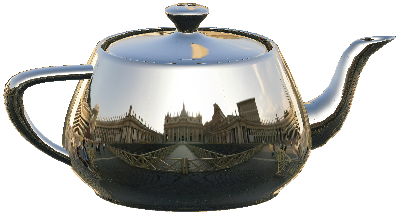
\includegraphics[height=5cm]{cubemap1.png} }}%
    \subfloat[]{{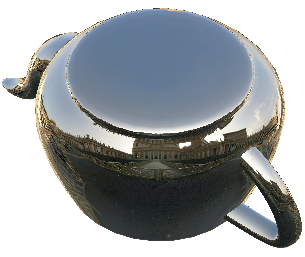
\includegraphics[height=5cm]{cubemap2.png} }}%
\end{figure}







































%